% (c) 2017 Daniele Zambelli - daniele.zambelli@gmail.com
% 
% Tutti i grafici per il capitolo relativo al calcolo combinatorio
%

\newcommand{\dadomonetacart}{%
  \def \mix{0}
  \def \max{7}
  \def \miy{0}
  \def \may{7}
  \disegno{
    \rcomvar{\mix}{\max}{\miy}{\may}{gray!50, very thin, step=1}{M}{D}
    \foreach \ux in {1, ..., 6} {
      \node at (\ux, 0) [below] {\(\ux\)};
      \foreach \uy in {1, 2} {
        \fill (\ux, \uy) circle(2pt);}}
    \foreach \uy/\ly in {1/T, 2/C} {
      \node at (0, \uy) [left] {\(\ly\)};}
  }
}

\newcommand{\monetadadocart}{%
  \def \mix{0}
  \def \max{7}
  \def \miy{0}
  \def \may{7}
  \disegno{
    \rcomvar{\mix}{\max}{\miy}{\may}{gray!50, very thin, step=1}{M}{D}
    \foreach \ux/\lx in {1/T, 2/C} {
      \node at (\ux, 0) [below] {\(\lx\)};
      \foreach \uy in {1, ..., 6} {
        \fill (\ux, \uy) circle(2pt);}}
    \foreach \uy in {1, ..., 6} {
      \node at (0, \uy) [left] {\(\uy\)};}
  }
}

\newcommand{\monetadadoalbero}{%
  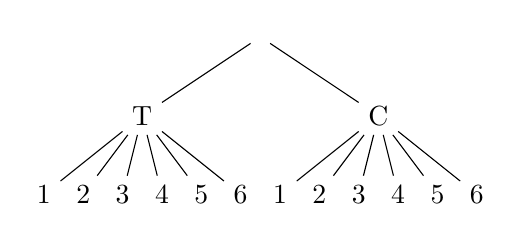
\begin{tikzpicture}[level distance=1.0cm,
    level 1/.style={sibling distance=3cm},
    level 2/.style={sibling distance=0.5cm}]
    \node {}
      child {node {T}
        child {node {1}}
        child {node {2}}
        child {node {3}}
        child {node {4}}
        child {node {5}}
        child {node {6}}
      }
      child {node {C}
        child {node {1}}
        child {node {2}}
        child {node {3}}
        child {node {4}}
        child {node {5}}
        child {node {6}}
      };
  \end{tikzpicture}
}

\newcommand{\dadomonetaalbero}{%
  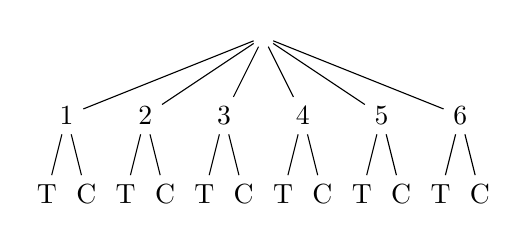
\begin{tikzpicture}[level distance=10mm,
    level 1/.style={sibling distance=10mm},
    level 2/.style={sibling distance=5mm}]
    \node {}
      child {node {1}
        child {node {T}}
        child {node {C}}
      }
      child {node {2}
        child {node {T}}
        child {node {C}}
      }
      child {node {3}
        child {node {T}}
        child {node {C}}
      }
      child {node {4}
        child {node {T}}
        child {node {C}}
      }
      child {node {5}
        child {node {T}}
        child {node {C}}
      }
      child {node {6}
        child {node {T}}
        child {node {C}}
      };
  \end{tikzpicture}
}
